\chapter{Mengenal Kecerdasan Buatan dan Scikit-Learn}
Buku umum teori lengkap yang digunakan memiliki judul\textit{Artificial intelligence: a modern approach}\cite{russell2016artificial}.  
Untuk pratikum sebelum UTS menggunakan buku \textit{Python Artificial Intelligence Projects for Beginners}\cite{eckroth2018python}. Buku pelengkap penunjang penggunaan python menggunakan buku \textit{Python code for Artificial Intelligence: Foundations of Computational Agents}\cite{poole2017python}.
Dengan praktek menggunakan python 3 dan editor anaconda dan library python scikit-learn.
Tujuan pembelajaran pada pertemuan pertama antara lain:
\begin{enumerate}
\item
Mengerti definisi kecerdasan buatan, sejarah kecerdasan buatan, perkembangan dan penggunaan di perusahaan
\item
Memahami cara instalasi dan pemakaian sci-kit learn
\item
Memahami cara penggunaan variabel explorer di spyder
\end{enumerate}
Tugas dengan cara dikumpulkan dengan pull request ke github dengan menggunakan latex pada repo yang dibuat oleh asisten riset.

\section{Teori}
Praktek teori penunjang yang dikerjakan :
\begin{enumerate}
\item Resume Definisi, Sejarah dan perkembangan Kecerdasan Buatan
	\begin{enumerate}
	\item Definisi Kecerdasan Buatan
	\newline Kecerdasan Buatan merupakan teknologi yang memiliki kecerdasan layaknya manusia namun kecerdasan yang dimiliki oleh AI merupakan hasil dari permodelan oleh manusia yang dibuat agar bisa berpikir seperti manusia.
	\item Sejarah Kecerdasan Buatan
	\newline Kecerdasan Buatan (Artificial Intelligence) bermula dari adanya kemunculan komputer pada tahun 1940, dengan salah satu penemuan model matematis bernama perceptron dari neuron didalam otak yang diusulkan oleh McMulloh dan Pitts di tahun 1943, dengan menunjukan bagaimana cara neuron menjadi aktif seperti saklar on/off dan neuron tersebut mampu memahami dan memberikan aksi terhadap dari waktu dari input yang diberikan. dibeberapa tahun kemudian ada beberapa penemuan dari beberapa ahli lainnya, seperti;
		\begin{itemize}
		 \item pada tahun 1950 - Paper berjudul Computing Machineri and Intelligence - dirancang oleh Alan Turing
		 \item pada tahun 1955 - The Logic Theorist - dirancang oleh Newell dan Simon
		 \item pada tahun 1956 s/d 1980 - pengembangan pemahaman mengenai AI dengan diadakannya konferensi dan diskusi dengan para ahli komputer
		\end{itemize}
	\item Perkembangan Kecerdasan Buatan
	\newline Perkembangan Kecerdasan Buatan, berkembang semenjak tahun 1956 - 1970, dengan dilakukan pemahaman dengan berdiskusi dengan para ahli komputer, banyak universitas juga yang berpartisipasi di MIT, seperti (universitas di Edinburgh, Standford dan Carnegie Mellon) yang mana komputer pemrograman mulai membuktikan masalah aljabar, teorema geometris yang menggunakan pemahaman sintaks dan tata bahasa inggris.
	\end{enumerate}
\item Resume mengenai definisi supervised learning, klasifikasi, regresi dan unsupervised learning Data set, training set dan testing set.
	\begin{enumerate}
	\item Definisi Supervised Learning, klasifikasi, regresi
		\begin{itemize}
		\item Definisi Supervised Learning
		\newline merupakan \emph{Machine Learning}  model yang mempelajari data dengan label atau target dimana evaluasi model tersebut akan berdasarkan target. contoh: pengenalan jenis bunga berdasarkan ukuran kelopak dan warna kelopak.
		\item Definisi Klasifikasi
		\newline merupakan \emph{Machine Learning}  model yang mempelajari data dengan label atau target dimana evaluasi model tersebut akan berdasarkan target. label merupakan pengenal dari sebuah data. contoh: pengenalan jenis bunga berdasarkan ukuran kelopak dan warna kelopak.
		\item Definisi Regresi
		\newline metode pada supervised learning yang mengembalikan target numerik untuk setiap sampel sedangkan klasifikasi adalah metode supervised learning yang bekerja dengan cara memberikan label pada setiap sampel dengan memilih dua atau lebih kelas atau kelompok yang berbeda.
		\end{itemize}
	\item Definisi Unspervised Learning, Dataset, Training Set dan Testing Set
		\begin{itemize}
		\item Definisi Unsupervised Learning
		\newline Unsupervised learning adalah salah satu tipe algoritma machine learning yang digunakan untuk menarik kesimpulan dari dataset
		\item Definisi Dataset
		\newline Dataset adalah istilah informal yang merujuk pada kumpulan . Secara umum, dataset berisi lebih dari satu variabel dan menyangkut suatu topik tertentu yang akan digunakan untuk klasifikasi dengan metode data mining. 
		\item Definisi Training Set
		\newline Training Set merupakan bagian dataset yang disiapkan untuk melatih model dalam membuat prediksi atau menjalankan fungsi dari sebuah algoritma ML. Kita memberikan petunjuk melalui algoritma agar mesin yang kita latih bisa mencari korelasinya sendiri atau belajar pola dari data yang diberikan.
		\item Definisi Testing Set
		\newline Testing Set merupakan bagian dataset yang disiapkan untuk melakukan tes pada model yang telah dilatih untuk melihat keakuratannya, atau dengan kata lain melihat performanya.
		\end{itemize}
	\end{enumerate}
\end{enumerate}

\section{Instalasi}
Membuka https://scikit-learn.org/stable/tutorial/basic/tutorial.html. Dengan menggunakan bahasa yang mudah dimengerti dan bebas plagiat. 
Dan wajib skrinsut dari komputer sendiri.
\newline Link Livestreaming: \href{https://youtu.be/sJbFyIBI_Jk}{Klik Disini}
\begin{enumerate}
\item
Instalasi library scikit dari anaconda, mencoba kompilasi dan uji coba ambil contoh kode dan lihat variabel explorer[hari ke 1](10)
\begin{figure}[!htbp]
    \centering
	\caption{Instalasi Sklearn Melalui Anaconda Prompt}
   	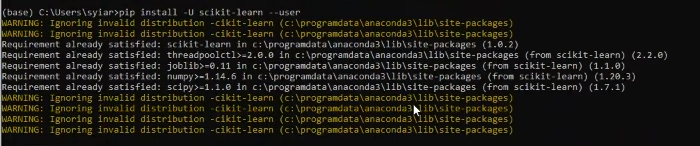
\includegraphics[scale=0.4]{figures/chapter 1/instalasi/1/cmdInstalasiSklearn.PNG}
	\caption{Variable Explorer}
	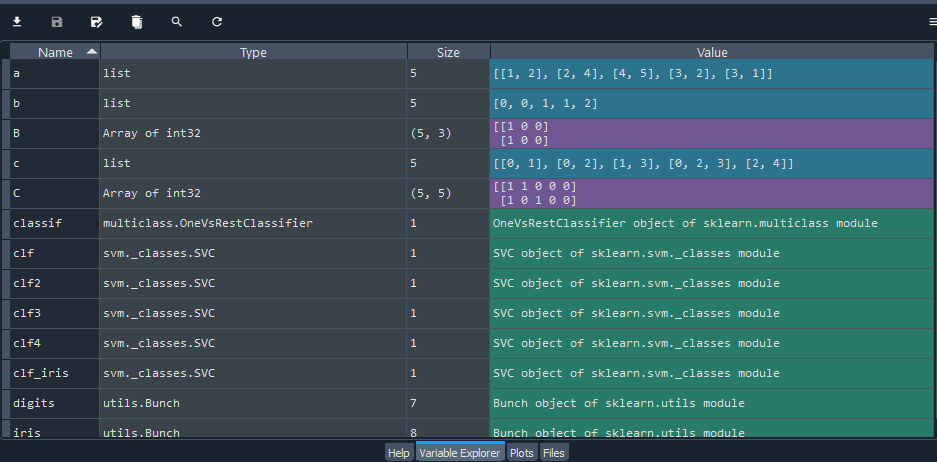
\includegraphics[scale=0.4]{figures/chapter 1/instalasi/1/variableExplorer.PNG}
\end{figure}
\item
Mencoba Loading an example dataset, menjelaskan maksud dari tulisan tersebut dan mengartikan per baris[hari ke 1](10)
\begin{figure}[!htbp]
    \centering
   	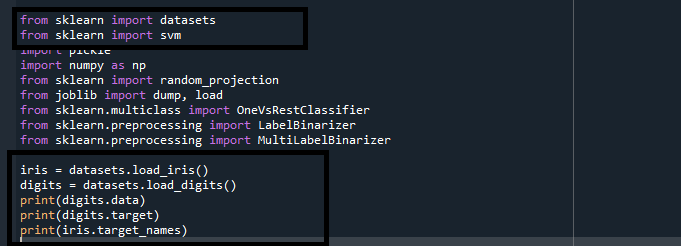
\includegraphics[scale=0.4]{figures/chapter 1/LoadDataset/SourceCode.PNG}
	\caption{Source Code Loading an example dataset}
	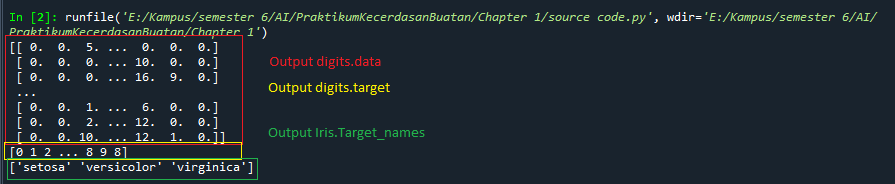
\includegraphics[scale=0.4]{figures/chapter 1/LoadDataset/OutputExampleDatasets.PNG}
	\caption{Output Example Dataset}
	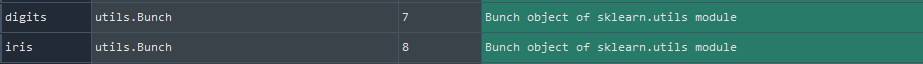
\includegraphics[scale=0.3]{figures/chapter 1/LoadDataset/VariableExplorerDataset.PNG}
	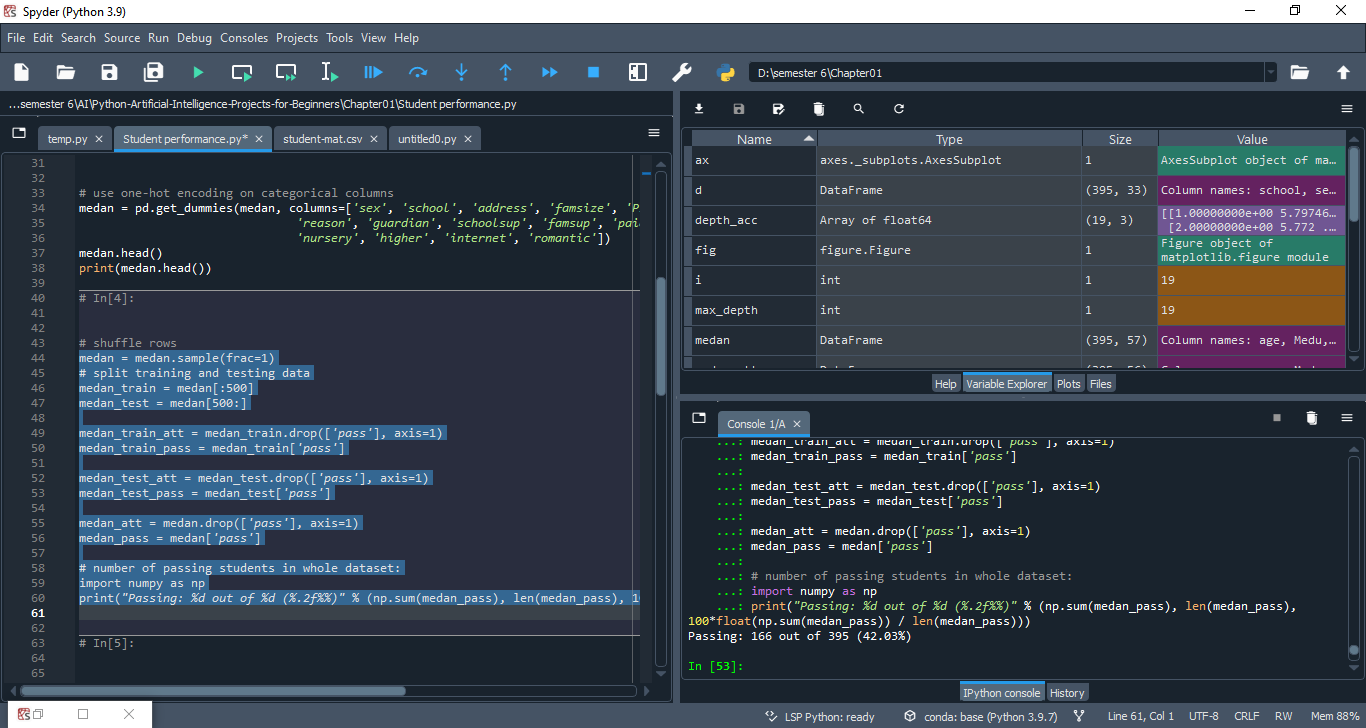
\includegraphics[scale=0.3]{figures/chapter 1/LoadDataset/4.PNG}
	\vspace{0.5cm}
	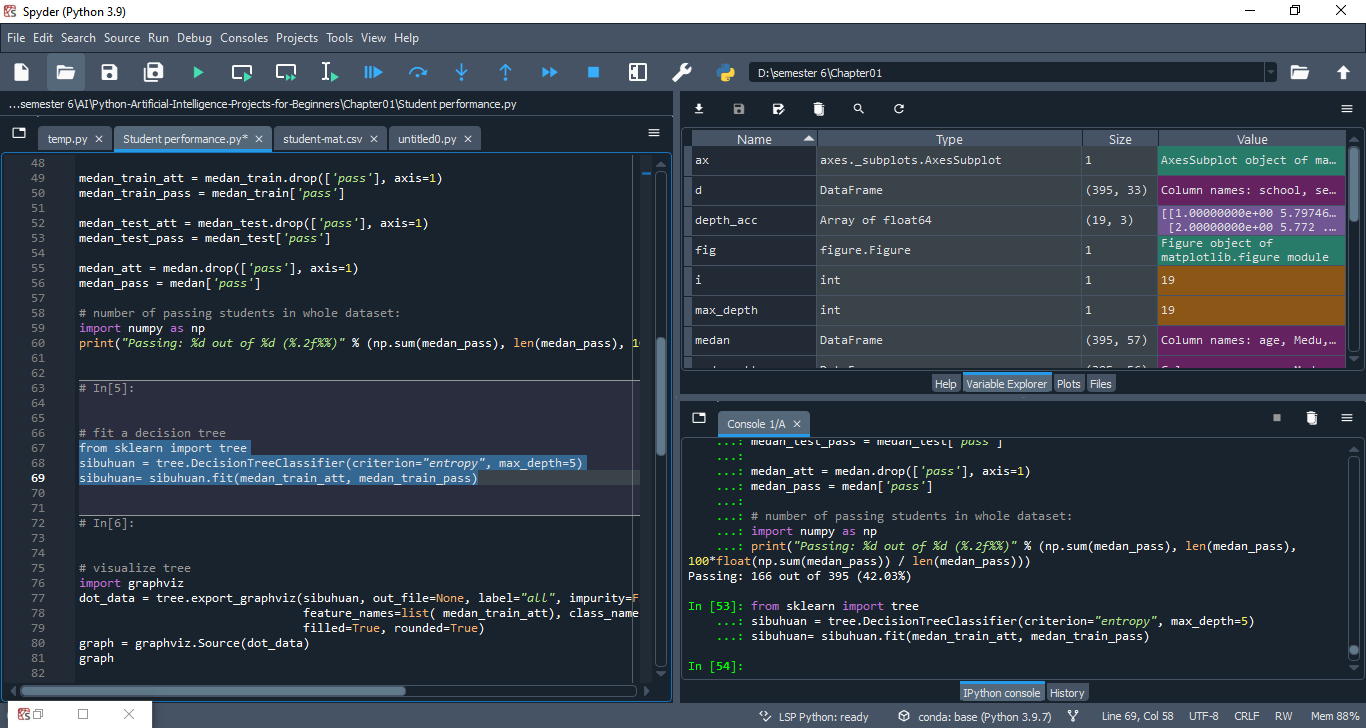
\includegraphics[scale=0.3]{figures/chapter 1/LoadDataset/5.PNG}
	\caption{Variable Explorer dari output dataset}
\end{figure}
\item
Mencoba Learning and predicting, menjelaskan maksud dari tulisan tersebut dan mengartikan per baris[hari ke 2](10)
\begin{figure}[!htbp]
    \centering
   	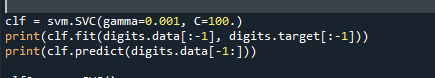
\includegraphics[scale=0.5]{figures/chapter 1/3/1.PNG}
	\caption{Source Code Learning and Predicting}
	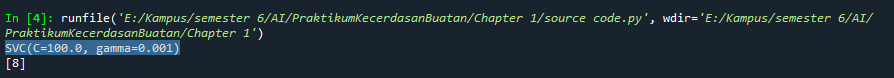
\includegraphics[scale=0.5]{figures/chapter 1/3/2.PNG}
	\caption{Output Learning and Predicting}
\end{figure}
\item
mencoba Model persistence, menjelaskan maksud dari tulisan tersebut dan mengartikan per baris[hari ke 2](10)
\begin{figure}[!htbp]
    \centering
   	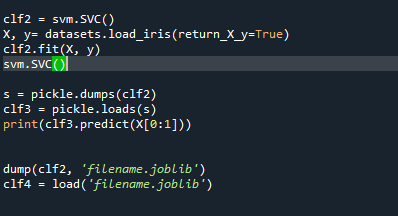
\includegraphics[scale=0.5]{figures/chapter 1/4/1.PNG}
	\caption{Source Code Model Persistence}
	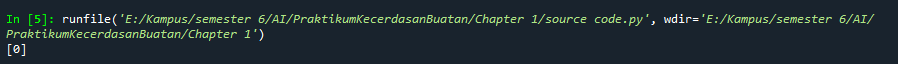
\includegraphics[scale=0.5]{figures/chapter 1/4/2.PNG}
	\caption{Output Menggunakan Pickle}
	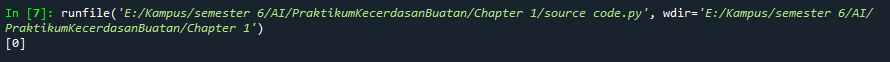
\includegraphics[scale=0.5]{figures/chapter 1/4/3.PNG}
	\caption{Output Menggunakan Joblib}
\end{figure}
\newpage
\item 
Mencoba Conventions, menjelaskan maksud dari tulisan tersebut dan mengartikan per baris[hari ke 2](10)
	\begin{figure}[!htbp]
	    \centering
	   	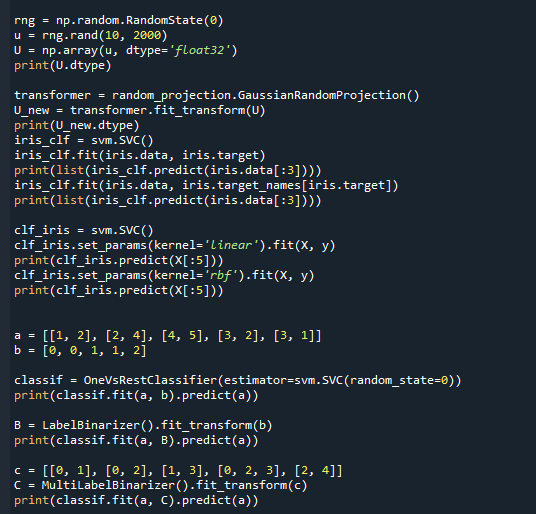
\includegraphics[scale=0.5]{figures/chapter 1/5/1.PNG}
		\caption{Source Code Convention}
		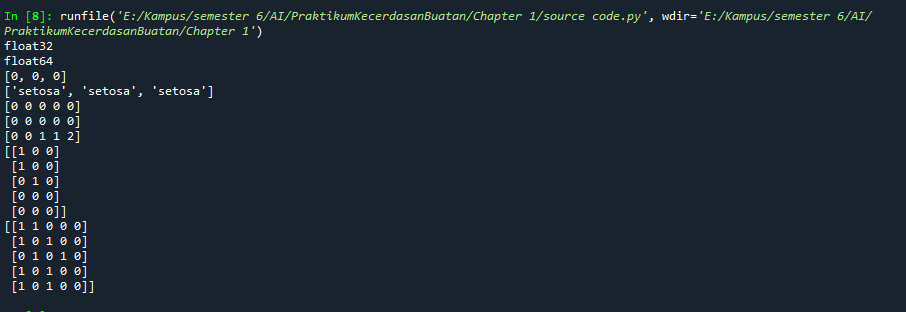
\includegraphics[scale=0.5]{figures/chapter 1/5/2.PNG}
		\caption{Output Source Code}
	\end{figure}
\end{enumerate}

\newpage
\section{Penanganan Error}
Dari percobaan yang dilakukan di atas, apabila mendapatkan error maka:
\begin{enumerate}
	\item
	skrinsut error[hari ke 2](10)
	\begin{figure}[!htbp]
	    \centering
	   	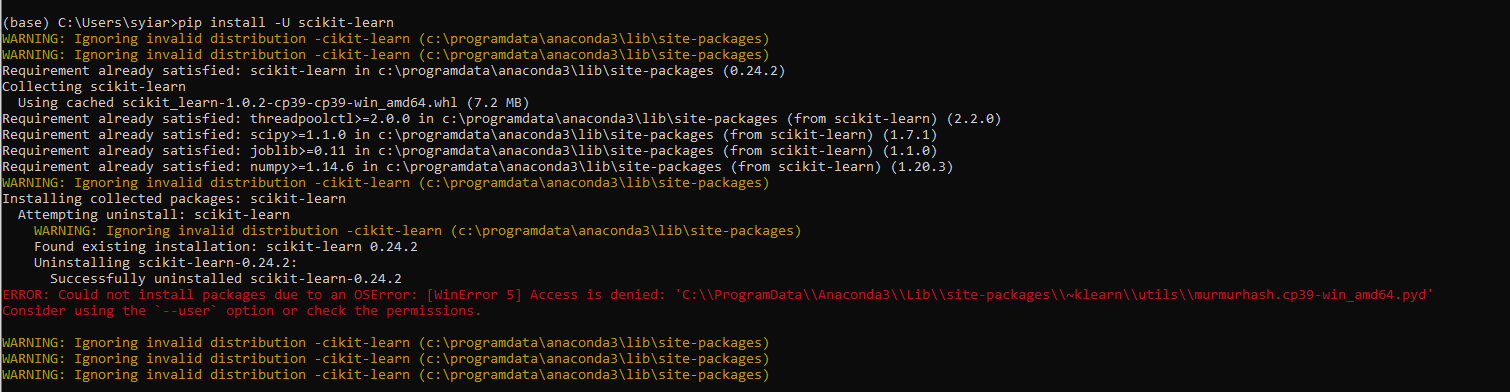
\includegraphics[scale=0.4]{figures/chapter 1/error/1.PNG}
		\caption{Error Could Not Install Packages due to an OSError Acces Is Denied}
	\end{figure}
	\item Tuliskan Kode error dan Jenis Errornya [hari ke 2](10)
	\newline pip install -U scikit-learn (jenis error Could Not Install Packages due to an OSError Acces Is Denied)
	\item Solusi pemecahan masalah error tersebut[hari ke 2](10)
	\newline tambahkan --user pada command install pip " pip install -U scikit-learn --user "
\end{enumerate}
